\section{Details on phase b.) of forecasting-based algorithms}\label{sec:forecasting-eval}
As noted in \cref{subsect:how-are-we-retrieving-it}, the evaluation of forecasting
errors is not part of (most) available forecasting packages. Therefore, a variety
of approaches was adopted for this paper. Most trivially, a moving mean and standard
deviation were used as a dynamic threshold. Every forecasting error exceeding this
threshold was remarked as a detection (\cref{def:detection}). Both 
\begin{enumerate*}
    \item using an \gls{ocsvm} and 
    \item identifying the best fitting distribution, then performing p-tests was
    disregarded for every forecasting error
\end{enumerate*}
were disregarded for their computational complexity and subpar results.

More complex scoring methods from \cite{Ahmad.2017,Hundman.2018} were adopted.

\textcite{Ahmad.2017} suggest to model the distribution of errors as a rolling normal
distribution with mean and standard deviation \(\mu_t, \sigma_t\) according to
\cref{eq:rolling-mean,eq:rolling-std}

\begin{align}
    \mu_t&= \frac{\sum_{i=0}^{i=W-1}s_{t-i}}{W}\label{eq:rolling-mean}\\
    \sigma_t &= \frac{\sum_{i=0}^{i=W-1}{(s_{t-i}-\mu_t)}^2}{W - 1}\label{eq:rolling-std}
\end{align}
where:
\begin{conditions}
    W &:= & Window size, set to \(W=8000\) as proposed by~\cite{Ahmad.2017}
\end{conditions}

and a short term rolling average \(\tilde{\mu}_t\) according to \cref{eq:short-rolling-mean}.

\begin{equation}
    \tilde{\mu}_t = \frac{\sum_{i=0}^{i=W'-1}s_{t-i}}{W'}\label{eq:short-rolling-mean}\\
\end{equation}
where:
\begin{conditions}
    W' &:= & Short-term window size, set to \(W'=10\) as proposed by~\cite{Ahmad.2017}
\end{conditions}

The likelihood (\cref{eq:likelihood}is calculated using the \gls{cdf} of a normal gaussian distribution
given in \cref{eq:cdf}
as
\begin{align}
    L_t &= \text{CDF}\left(\frac{\tilde{\mu}_t - \mu_t}{\sigma_t}\right)\label{eq:likelihood}\\
    \text{CDF}(x) &= \frac{1}{2} \left(1 + \text{erf}(\frac{x-\mu}{\sqrt{2\sigma}})\right)\label{eq:cdf}
\end{align}
where:
\begin{conditions}
    \mu&= & 0\\
    \sigma&= & 1\\
    \text{erf} &:= & the gaussian error function
\end{conditions}
Finally, a detection is recorded, when \(L_t \geq \epsilon \lor L_t \leq 1 - \epsilon\).
This is a slight deviation from~\cite{Ahmad.2017}, where only an upper p-test is
performed.

For details on the non-parametric thresholding as per \textcite{Hundman.2018},
please review their paper.


\section{Calculation of the Numenta Anonamly Metric Score}\label{app:numenta-score}
The Numenta Anomaly Metric Score for a single time series is the addition of
\begin{enumerate}[a.)]
    \item the sum of scores for every \defref{def:detection} (given by \cref{eq:score-per-detection}) and 
    \item the score for missed anomaly windows (false negatives) (given by \cref{eq:score-per-fn}).
\end{enumerate}

\begin{align}
    \sigma(t)&= \left(W_{TP} - W_{FP}\right) \left(\frac{1}{1 + e^{5t}}\right) - 1\label{eq:score-per-detection}\\
    \phi(F)&= W_{FN} * \bigl|F\bigr|\label{eq:score-per-fn}\\
    \text{Score}&= \left(\sum_{t\in T}{\sigma(t)}\right) + \phi(F)\label{eq:score-final}
\end{align}
where:
\begin{conditions}
    t &:= & the relative timestamp/position of the detection within the window.\\
    W_{\left\{TP, FP, FN\right\}} &:= & the weights attributed to true and false positives and false negatives respectively.\\
    F &:= & the set of false positives (anomaly windows without any detections).\\
    T &:= & the set of time stamps associated with the detections.
\end{conditions}

The final score per time series is calculated by \cref{eq:score-final}~\cite[cf][]{Lavin.2015}.
An example of the scoring function can be seen in \cref{fig:anomaly-score-example}.

\begin{figure}[htp!]
    \centering
    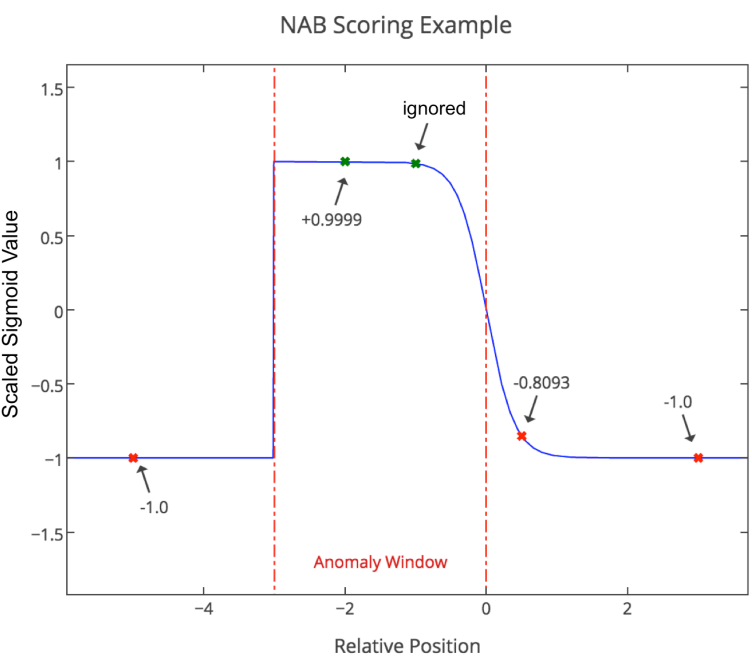
\includegraphics[width=.6\textwidth]{anomaly_scoring.png}
    \caption[Example of anomaly scoring function]{Example application of the anomaly
    scoring function. Illustration adopted from~\cite{Lavin.2015}. The following
    text (blue) is cited from \textcite{Lavin.2015}:
    {\color{blue}
    Scoring example for a sample anomaly window, where the values
    represent the scaled sigmoid function, the second term in \cref{eq:score-per-detection}.
    The first point is an FP preceding the anomaly window (red dashed lines) and
    contributes -1.0 to the score. Within the window we see two detections, and
    only count the earliest TP for the score. There are two FPs after the window.
    The first is less detrimental because it is close to the window, and the second
    yields -1.0 because it’s too far after the window to be associated with the true
    anomaly. TNs make no score contributions. The scaled sigmoid values are
    multiplied by the relevant application profile weight, as shown in Eq.,
    the NAB score for this example would calculate as: 
    \(-1.0W_{FP} + 0.9999W_{TP} - 0.8093W_{FP} - 1.0W_{FP}\).
    With the standard application profile this would result in a total score of
    \(0.6909\).}
    }\label{fig:anomaly-score-example}
\end{figure}\clearpage

\section{Additional Plots of the Datasets}\label{sect:additonal-plots-dataset}
This section provides additional time series plots from \gls{nab}.
% Artificial Data art_daily_flatmiddle  art_daily_jumpsdown art_daily_nojump art_load_balancer_spikes
\begin{figure}[htp!]
    \centering
    \begin{subfigure}[t]{.49\linewidth}
        \centering
        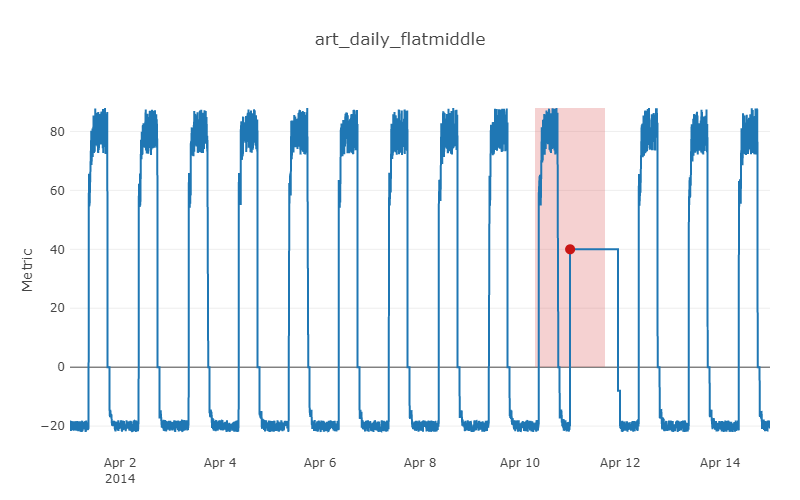
\includegraphics[width=\textwidth]{anomaly_types_examples/final/png/art_daily_flatmiddle.png}
        \subcaption{art\_daily\_flatmiddle.csv}\label{app-fig:art_daily_flatmiddle}
    \end{subfigure}
    \begin{subfigure}[t]{.49\linewidth}
        \centering
        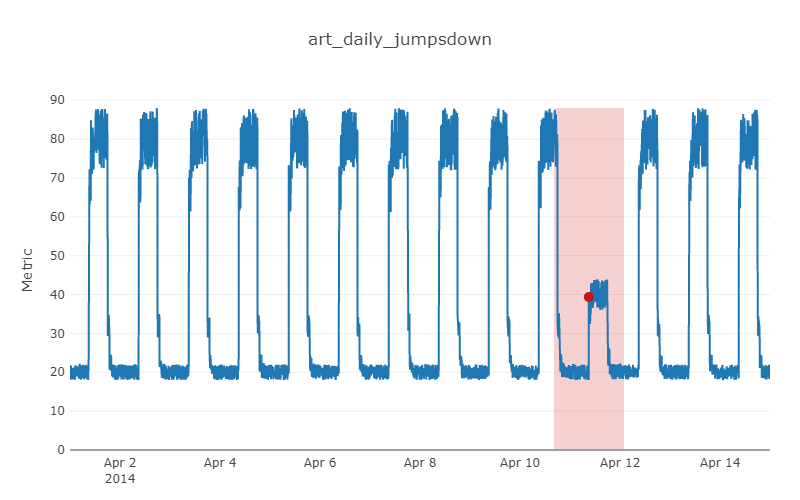
\includegraphics[width=\textwidth]{anomaly_types_examples/final/png/art_daily_jumpsdown.png}
        \subcaption{art\_daily\_jumpsdown.csv}\label{app-fig:art_daily_jumpsdown}
    \end{subfigure}
    \begin{subfigure}[t]{.49\linewidth}
        \centering
        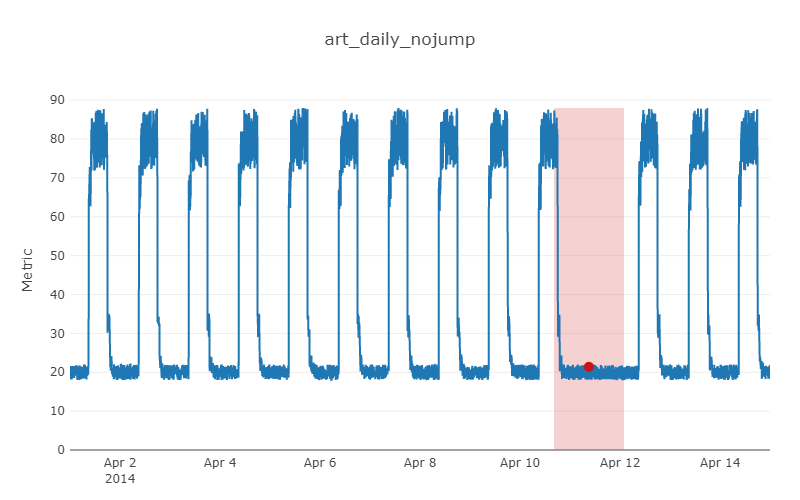
\includegraphics[width=\textwidth]{anomaly_types_examples/final/png/art_daily_nojump.png}
        \subcaption{art\_daily\_nojump.csv}\label{app-fig:art_daily_nojump}
    \end{subfigure}
    \begin{subfigure}[t]{.49\linewidth}
        \centering
        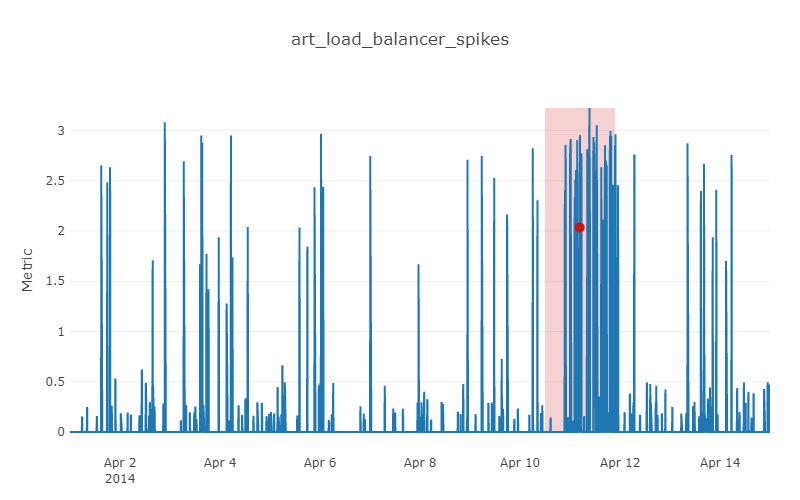
\includegraphics[width=\textwidth]{anomaly_types_examples/final/png/art_load_balancer_spikes.png}
        \subcaption{art\_load\_balancer\_spikes.csv}\label{app-fig:art_load_balancer_spikes}
    \end{subfigure}
    \caption{Artificial anomaly samples}\label{app-fig:artificial-anomaly-types-nab}
\end{figure}
% Mean: ec2_cpu_utilization_53ea38 grok_asg_anomaly
\begin{figure}[htp!]
    \centering
    \begin{subfigure}[t]{.49\linewidth}
        \centering
        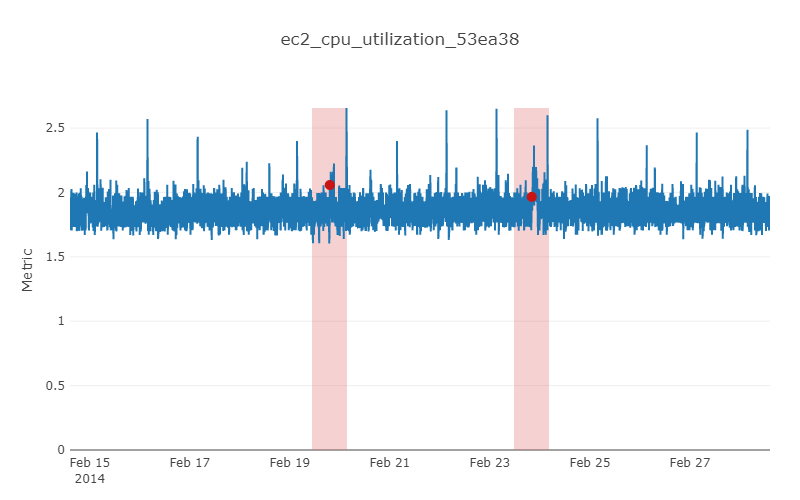
\includegraphics[width=\textwidth]{anomaly_types_examples/final/png/ec2_cpu_utilization_53ea38.png}
        \subcaption{ec2\_cpu\_utilization\_53ea38.csv}\label{app-fig:ec2_cpu_utilization_53ea38}
    \end{subfigure}
    \begin{subfigure}[t]{.49\linewidth}
        \centering
        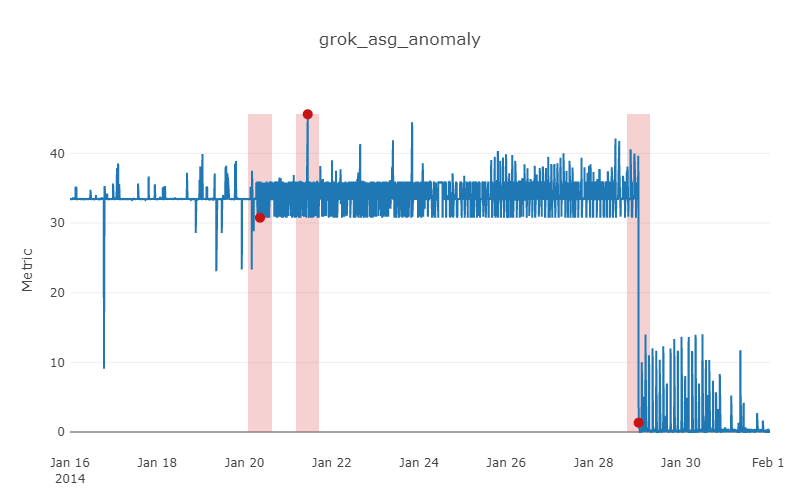
\includegraphics[width=\textwidth]{anomaly_types_examples/final/png/grok_asg_anomaly.png}
        \subcaption{grok\_asg\_anomaly.csv}\label{app-fig:grok_asg_anomaly}
    \end{subfigure}
    \caption[Contextual anomalies and change points]{(\subref{app-fig:ec2_cpu_utilization_53ea38}) 
    shows contextual anomalies, (\subref{app-fig:grok_asg_anomaly}) shows two
    change points and a point-anomaly.}\label{fig:artificial-anomaly-types-nab}
\end{figure}
% Spikes:
% ec2_cpu_utilization_24ae8d ec2_network_in_5abac7 ec2_request_latency_system_failure elb_request_count_8c0756 Twitter_volume_CRM Twitter_volume_CVS Twitter_volume_KO ambient_temperature_system_failure
\begin{figure}[htp!]
    \centering
    \begin{subfigure}[t]{.49\linewidth}
        \centering
        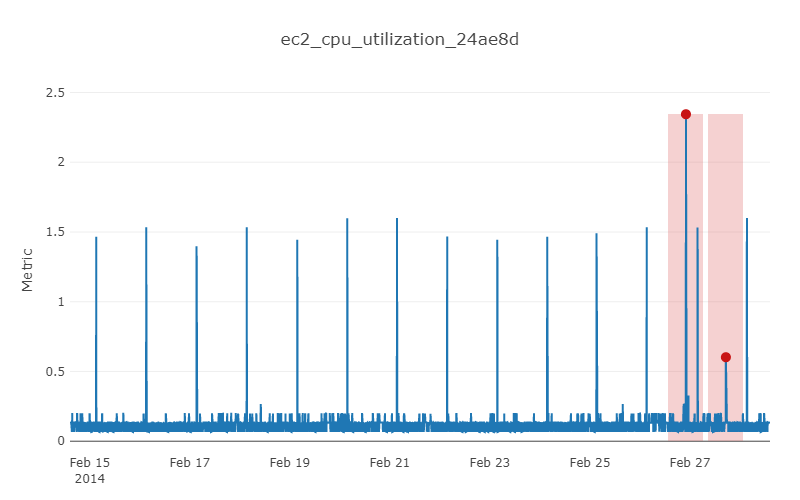
\includegraphics[width=\textwidth]{anomaly_types_examples/final/png/ec2_cpu_utilization_24ae8d.png}
        \subcaption{ec2\_cpu\_utilization\_24ae8d.csv}\label{app-fig:ec2_cpu_utilization_24ae8d}
    \end{subfigure}
    \begin{subfigure}[t]{.49\linewidth}
        \centering
        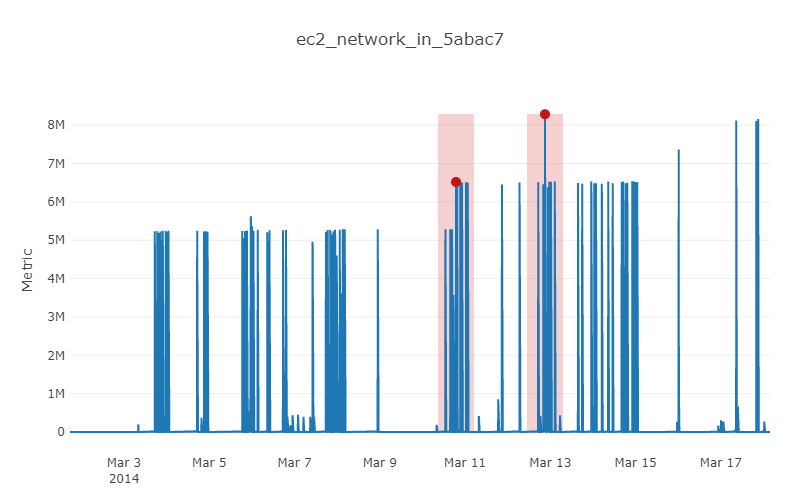
\includegraphics[width=\textwidth]{anomaly_types_examples/final/png/ec2_network_in_5abac7.png}
        \subcaption{ec2\_network\_in\_5abac7.csv}\label{app-fig:ec2_network_in_5abac7}
    \end{subfigure}
    \begin{subfigure}[t]{.49\linewidth}
        \centering
        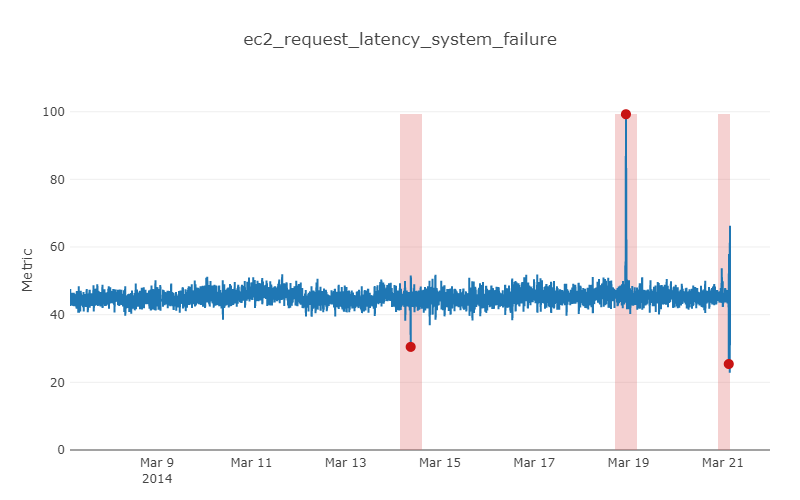
\includegraphics[width=\textwidth]{anomaly_types_examples/final/png/ec2_request_latency_system_failure.png}
        \subcaption{ec2\_request\_latency\_system\_failure.csv}\label{app-fig:ec2_request_latency_system_failure}
    \end{subfigure}
    \begin{subfigure}[t]{.49\linewidth}
        \centering
        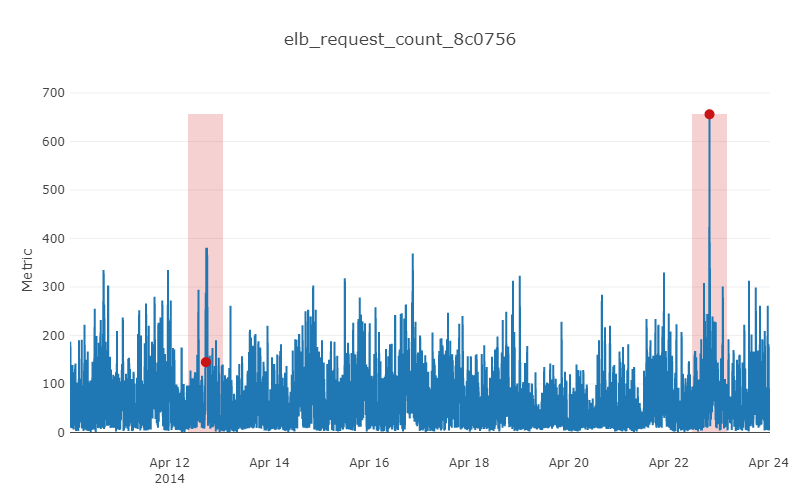
\includegraphics[width=\textwidth]{anomaly_types_examples/final/png/elb_request_count_8c0756.png}
        \subcaption{elb\_request\_count\_8c0756.csv}\label{app-fig:elb_request_count_8c0756}
    \end{subfigure}
    \begin{subfigure}[t]{.49\linewidth}
        \centering
        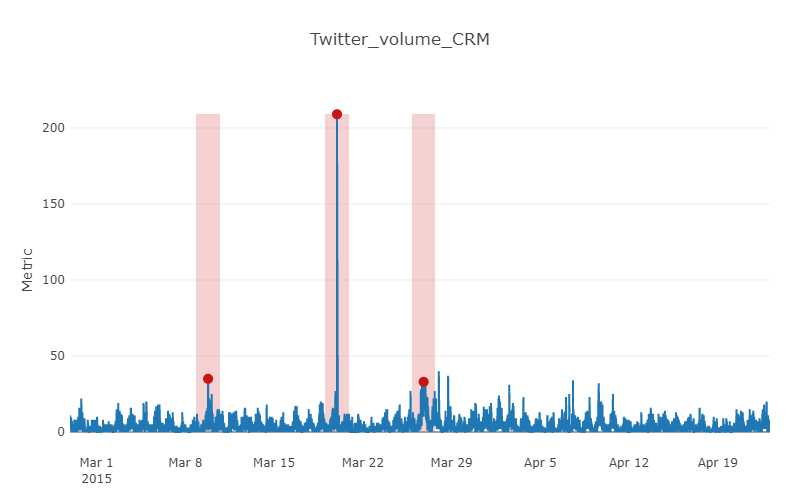
\includegraphics[width=\textwidth]{anomaly_types_examples/final/png/Twitter_volume_CRM.png}
        \subcaption{Twitter\_volume\_CRM.csv}\label{app-fig:Twitter_volume_CRM}
    \end{subfigure}
    \begin{subfigure}[t]{.49\linewidth}
        \centering
        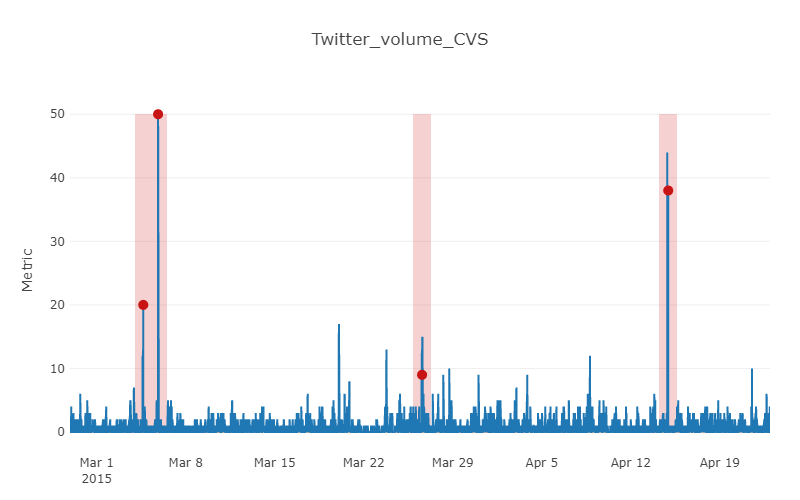
\includegraphics[width=\textwidth]{anomaly_types_examples/final/png/Twitter_volume_CVS.png}
        \subcaption{Twitter\_volume\_CVS.csv}\label{app-fig:Twitter_volume_CVS}
    \end{subfigure}
    \begin{subfigure}[t]{.49\linewidth}
        \centering
        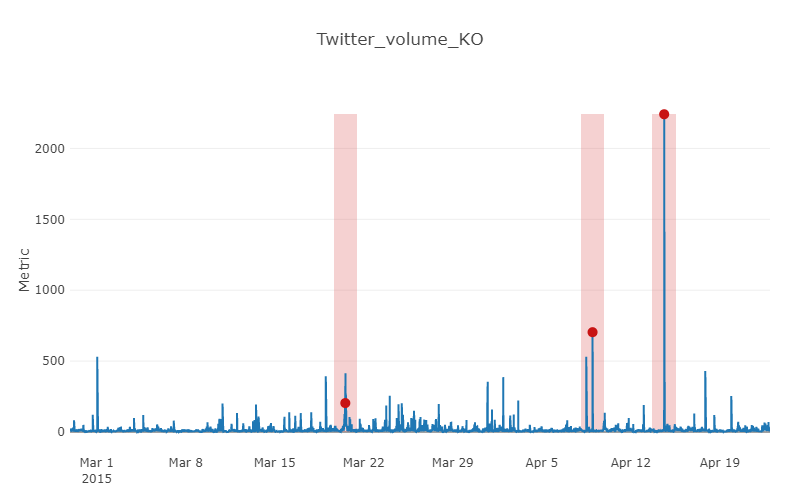
\includegraphics[width=\textwidth]{anomaly_types_examples/final/png/Twitter_volume_KO.png}
        \subcaption{Twitter\_volume\_KO.csv}\label{app-fig:Twitter_volume_KO}
    \end{subfigure}
    \begin{subfigure}[t]{.49\linewidth}
        \centering
        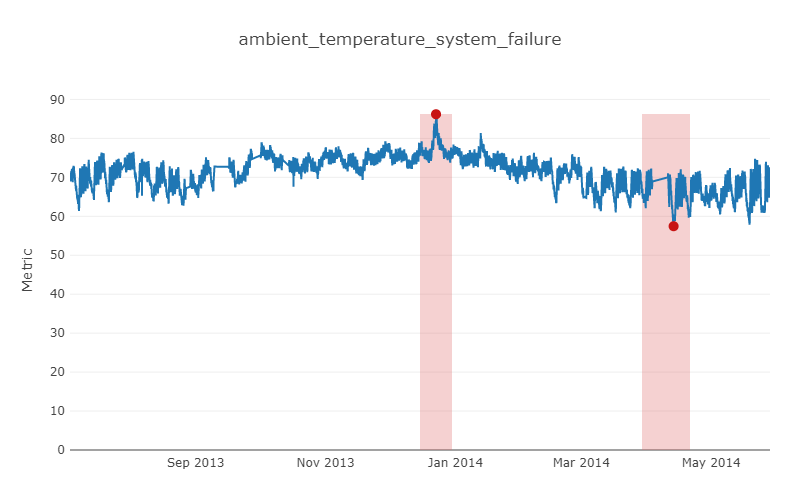
\includegraphics[width=\textwidth]{anomaly_types_examples/final/png/ambient_temperature_system_failure.png}
        \subcaption{ambient\_temperature\_system\_failure.csv}\label{app-fig:ambient_temperature_system_failure}
    \end{subfigure}
    \caption{Point Anomalies. All illustrations by the author.}\label{fig:spiking-types}
\end{figure}\clearpage



\section{Other Datasets}
% Table of several univariate datasets
\begin{table}[h]\centering
    \ra{1.3}
        \begin{tabular}{l}
            Dataset                                                                                                                             \\\midrule
            \href{https://github.com/numenta/NAB}{Numenta Anomaly Benchmark}                                                                    \\\addlinespace
            \href{https://www.kaggle.com/averkij/tennessee-eastman-process-simulation-dataset}{Tennessee Eastman Process Simulation Dataset}    \\\addlinespace
            \href{https://github.com/alan-turing-institute/TCPDBench}{Turing Change Point Benchmark}                                            \\\addlinespace
            \href{https://itrust.sutd.edu.sg/testbeds/secure-water-treatment-swat/}{Secure Water Treatment}                                     \\\addlinespace
            \href{https://en.wikipedia.org/wiki/Makridakis\_Competitions}{M-Competitions}                                                       \\\addlinespace
            \href{https://webscope.sandbox.yahoo.com/catalog.php?datatype=s\&did=70}{Yahoo! Webscope S5}                                        \\
        \end{tabular}
    \caption{Univariate Datasets}\label{tab:univariate-datasets}
\end{table}

% Table of several multivariate datasets
\begin{table}[h]\centering
    \ra{1.3}
        \begin{tabular}{l}
            Dataset                                                                                                                             \\\midrule
            \href{https://www.kaggle.com/anomalydetectionml/features}{Data from: Machine Learning-based Anomaly Detection in Software Systems}  \\\addlinespace
            \href{https://github.com/ricardovvargas/3w_dataset}{3W Dataset}                                                                     \\\addlinespace
            \href{https://www.kaggle.com/rkuo2000/nasa-bearing-sensor-data/notebooks}{NASA Bearing Sensor Data}                                 \\\addlinespace
            \href{https://github.com/chickenbestlover/RNN-Time-series-Anomaly-Detection}{HOT SAX Datasets}                                      \\\addlinespace
            \href{https://github.com/khundman/telemanom}{Soil Moisture Active Passive (SMAP)}                                                   \\\addlinespace
            \href{https://github.com/khundman/telemanom}{Mars Science Laboratory  (MSL)}                                                        \\\addlinespace
            \href{https://www.kaggle.com/icsdataset/hai-security-dataset}{HIL-based Augmented ICS}                                              \\
        \end{tabular}
        \caption{Multivariate-Datasets}\label{tab:multivariate-datasets}
\end{table}\clearpage


\section{Algorithm Selection}\label{sect:algorithms}
% Curation from
\begin{table}[h]\centering
    \ra{1.3}
        \begin{tabular}{l}
            Curated List                                                                                    \\\midrule                                                                               
            \url{https://github.com/cuge1995/awesome-time-series}                                           \\\addlinespace                                                                               
            \url{https://github.com/xephonhq/awesome-time-series-database}                                  \\\addlinespace
            \url{https://github.com/MaxBenChrist/awesome_time_series_in_python}                             \\\addlinespace
            \url{https://github.com/cuge1995/awesome-time-series}                                           \\\addlinespace
            \url{https://github.com/yzhao062/anomaly-detection-resources#34-time-series-outlier-detection}  \\\addlinespace
            \url{https://github.com/rob-med/awesome-TS-anomaly-detection}                                   \\\addlinespace
            \url{https://www.kaggle.com/general/185462}                                                     \\
        \end{tabular}
    \caption{Curated lists for open source anomaly detection libraries}\label{tab:curation-lists}
\end{table}

% Libraries for anomaly detection
\begin{table}[h]\centering
    \ra{1.3}
    \resizebox{\textwidth}{!}{%
        \begin{tabular}{lllll}
            Library                                                                                                 & Models    & Version   & Latest Commit     & Stars \\\midrule
            \href{https://github.com/arundo/adtk}{Anomaly Detection Toolkit (ADTK)}                                 & \makecell[l]{Statistical Models:\\\tabitem AR\\\tabitem Seasonal Pattern/Decomposition\\\tabitem Generalized ESD-Test\\\tabitem Difference in Mean\\\tabitem Difference in QR/IQR\\\tabitem Difference in Volatility; \\\\ML:\\\tabitem Clustering}                                                                                                                                                                           & 0.6.2     & 17th April 2020   & 582   \\\addlinespace
            \href{https://github.com/smirmik/CAD}{Contextual Anomaly Detector}                                      & No Documentation. Winner of NAB 2016                                                                                                                                                                                                                                                                                                                                                                                          & /         & 10th August 2016  & 63    \\\addlinespace
            \href{https://github.com/MentatInnovations/datastream.io}{datastream.io}                                & \makecell[l]{Focused on integration into ELK-stack;\\ Gaussian-Distribution and Difference in Percentile}                                                                                                                                                                                                                                                                                                                     & /         & 20th Feb 2018     & 804   \\\addlinespace 
            \href{https://github.com/NetManAIOps/donut}{DONUT}                                                      & Variational Auto-Encoder~\cite{Xu.2018}                                                                                                                                                                                                                                                                                                                                                                                       & /         & 6th March         & 298   \\\addlinespace 
            \href{https://github.com/hastic}{hastic}                                                                & \makecell[l]{Focused on Grafana.\\Thresholding on seasonality adjusted and exponentially smoothed data.}                                                                                                                                                                                                                                                                                                                      & /         & 26th Dec 2020     & 274   \\\addlinespace 
            \href{https://github.com/linkedin/luminol}{luminol}                                                     & Bitmap-Transformation~\cite{Wei.2005}, Single Exponential Smoothing;                                                                                                                                                                                                                                                                                                                                                          & 0.4       & 9th Jan 2018      & 861   \\\addlinespace 
            \href{https://github.com/datamllab/pyodds}{PyODDS} / \href{https://github.com/yzhao062/pyod}{PyOD}      & \makecell[l]{Statistical Models:\\\tabitem Local Outlier Factor\\\tabitem Clustering Based Local Outlier Factor\\\tabitem Histogram-Based Outlier Score\\\tabitem Isolation Forest\\\tabitem kNN\\\tabitem One-Class SVM\\\tabitem PCA\\\tabitem Robust Covariance\\\tabitem Subspace Outlier Detection\\\tabitem Luminol\\ Deep Learning:\\\tabitem LSTMAD\cite{Malhotra.2015}\\\tabitem DAGMM~\cite{Zong.2018}}             & /         & 8th May 2020      & 132   \\\addlinespace 
            \href{https://github.com/kLabUM/rrcf}{rrcf}                                                             & Robust Random Cut Forest~\cite{Guha.2016}                                                                                                                                                                                                                                                                                                                                                                                     & 0.4.3     & 10th June 2020    & 271   \\\addlinespace 
            \href{https://github.com/chickenbestlover/RNN-Time-series-Anomaly-Detection}{rnn ts anomaly detection}  & LSTM, GRU, SRU                                                                                                                                                                                                                                                                                                                                                                                                                & /         & 21st Oct 2020     & 684   \\\addlinespace 
            \href{https://github.com/datamllab/tods}{TODS: Time-series Outlier Detection System}                    & DeepLog~\cite{Du.2017}, Telemanom Matrix Profile, PyOD algorithms                                                                                                                                                                                                                                                                                                                                                             & /         & 5th Jan 2021      & 258   \\\addlinespace
            \href{https://github.com/earthgecko/skyline}{Skyline}                                                   & Ensemble of statistical tests like Kolmogorov-Smirnov, Grubbs, deviation from median\ldots                                                                                                                                                                                                                                                                                                                                    & 2.0       & 22th Dec 2020     & 284   \\\addlinespace
            \href{https://github.com/tsurubee/banpei}{Banpei}                                                       & Hotelling's theory~\cite{Hotelling.1990} and Singular Spectrum Transformation                                                                                                                                                                                                                                                                                                                                                 & /         & 21st Sept 2020    & 222   \\\addlinespace
            \href{https://github.com/htm-community/htm.core}{NuPIC}                                                 & Numenta HTM                                                                                                                                                                                                                                                                                                                                                                                                                   & /         & 23 Oct 2019       & 6.2k   \\\addlinespace
            \href{https://github.com/matrix-profile-foundation/matrixprofile}{MPF}                                  & Matrix Profile                                                                                                                                                                                                                                                                                                                                                                                                                & /         & 26th Dec 2020     & 121    \\
        \end{tabular}
    }
    \caption{Boundary Focused Detection Libraries, accessed last: 8th Jan 2021}\label{tab:ad-packages}
\end{table}


% Libraries for forecasting
\begin{table}[h]\centering
    \ra{1.3}
    \resizebox{\textwidth}{!}{%
        \begin{tabular}{lllll}
            Library                                                                                     & Models                                                                                                                                                                                                                                                                                                                            & Version   & Latest Commit         & Stars \\\midrule
            \href{https://github.com/firmai/atspy}{AtsPy}                                               & \makecell[l]{Conglomeration of independent libraries:\\\tabitem Auto ARIMA\\\tabitem Prophet\\\tabitem N-Beats\\\tabitem Gluon-TS\\\tabitem and TBAT;\\ Also:\\\tabitem Holt Winters}                                                                                                                                              & /         & 12th Nov 2020         & 320   \\\addlinespace
            \href{https://github.com/awslabs/gluon-ts}{GluonTS}                                         & \makecell[l]{Deep Learning:\\\tabitem Deep Factors for Forecasting~\cite{Wang.2019}\\\tabitem DeepAR~\cite{Flunkert.2017}\\\tabitem Deep State Space~\cite{Rangapuram.2018}\\\tabitem Gaussian Processes\\\tabitem N-Beats~\cite{Oreshkin.2020}\\\tabitem  Transformer\\\tabitem  Wavenet\\Also Includes:\\\tabitem  Prophet}     & 0.6.4     & 7th Jan 2021          & 1.7k  \\\addlinespace
            \href{https://github.com/alkaline-ml/pmdarima}{pmdarima}                                    & SARIMAX                                                                                                                                                                                                                                                                                                                           & 1.8       & 2nd December 2020     & 790   \\\addlinespace
            \href{https://github.com/RJT1990/pyflux}{PyFlux}                                            & ARIMAX, Dynamic AR, Dynamic Linear Regression, EARCH, GAS, ARCH, GARCH\ldots                                                                                                                                                                                                                                                      & /         & 16th December 2018    & 1.8k  \\\addlinespace
            \href{https://github.com/alan-turing-institute/sktime}{sktime}                              & ARIMA, Exponential Smoothing/Holt Winters, Polynomial Thresholding                                                                                                                                                                                                                                                                & 0.5.1     & 6th Jan 2021          & 3.4k  \\\addlinespace
            \href{https://github.com/bashtage/arch}{ARCH}                                               & AR, Heterogeneous Autoregression, ARCH, GARCH, TARCH, EGARCH, \ldots                                                                                                                                                                                                                                                              & 4.15      & 7th Jan 2021          & 630   \\\addlinespace
            \href{https://github.com/LongxingTan/Time-series-prediction}{Time Series Prediction TF2}    & LSTM, GRU, Wavenet, Transformer, N-Beats, GAN                                                                                                                                                                                                                                                                                     & /         & 25th December 2020    & 292   \\\addlinespace
            \href{https://github.com/maxjcohen/transformer}{Transformers for Timer Series}              & Transformer                                                                                                                                                                                                                                                                                                                       & 0.3       & 10th December 2020    & 231   \\\addlinespace
            \href{https://github.com/facebook/prophet}{Prophet}                                         & \makecell[l]{General Additive Model\\\tabitem trend is fitted via a logistic or a linear model\\\tabitem seasonality is fitted via Fourier series\\\tabitem also considers holidays}                                                                                                                                              & 0.6       & 7th Jan 2021          & 12.1k \\\addlinespace
            \href{https://github.com/intive-DataScience/tbats}{TBATS}                                   & Automated BATS/TBATS fitting                                                                                                                                                                                                                                                                                                      & 1.1       & 27th July 2020        & 84    \\\addlinespace
            \href{https://github.com/philipperemy/n-beats}{N-Beats}                                     & Res- and fully connected layer                                                                                                                                                                                                                                                                                                    & /         & 30th April 2020       & 326   \\
        \end{tabular}
    }
    \caption{Forecasting-Focused Libraries, accessed last: 8th Jan 2021}\label{tab:forecasting-packages}
\end{table}

% Chosen Library Anomaly Detection & Forecasting
\begin{table}[h]\centering
    \ra{1.3}
        \begin{tabular}{l}
            Boundary-Libraries \\\midrule
            \href{https://github.com/datamllab/pyodds}{PyODDS} / \href{https://github.com/yzhao062/pyod}{PyOD}      \\\addlinespace
            \href{https://github.com/kLabUM/rrcf}{rrcf}                                                             \\\addlinespace
            \href{https://github.com/earthgecko/skyline}{Skyline}                                                   \\\addlinespace
            \href{https://github.com/htm-community/htm.core}{NuPIC}                                                 \\\addlinespace\addlinespace
            Forecasting-Libraries \\\midrule
            \href{https://github.com/awslabs/gluon-ts}{GluonTS}                                                     \\\addlinespace
            \href{https://github.com/firmai/atspy}{AtsPy}                                                           \\\addlinespace
            \href{https://github.com/RJT1990/pyflux}{PyFlux}                                                        \\\addlinespace
            \href{https://github.com/alan-turing-institute/sktime}{sktime}                                          \\\addlinespace
        \end{tabular}
    \caption{Chosen Libraries}\label{tab:chosen-packages}
\end{table}

% Chosen Forecasting Algo
\begin{table}[h]\centering
    \ra{1.3}
        \begin{tabular}{ll}
            Forecasting Algorithm                                       & Package/Implementation    \\\midrule         
            Prophet~\cite{Taylor.2017}                                  & \href{https://github.com/firmai/atspy}{AtsPy}             \\\addlinespace
            Auto ARIMA~\cite{Smith.2017}                                & \href{https://github.com/alkaline-ml/pmdarima}{pmdarima}  \\\addlinespace
            ARIMA~\cite[Hyperparameters adopted from][]{Braei.2020}     & \href{https://github.com/alkaline-ml/pmdarima}{pmdarima}  \\\addlinespace
            Holt-Winters~\cite{Winters.1960}                            & \href{https://github.com/firmai/atspy}{AtsPy}             \\\addlinespace
            N-BEATS~\cite{Oreshkin.2020}                                & Implementation by the author                              \\\addlinespace
            TBAT/S                                                      & \href{https://github.com/firmai/atspy}{AtsPy}             \\\addlinespace
            DeepAnT~\cite{Munir.2019}                                   & Implementation by the author                              \\
        \end{tabular}
    \caption{Chosen Forecasting Algorithms}\label{tab:chosen-forecasting-algo}
\end{table}

% Chosen Boundary Algo
\begin{table}[h]\centering
    \ra{1.3}
        \begin{tabular}{ll}
            Boundary Algorithm                                  & Package/Implementation   \\\midrule                                                                               
            \gls{lof}~\cite{Breunig.2000}                       & \href{https://github.com/datamllab/pyodds}{PyODDS}                            \\\addlinespace
            Autoencoder~\cite[499\psqq]{Goodfellow.2016}        & \href{https://github.com/datamllab/pyodds}{PyODDS}                            \\\addlinespace
            \gls{cblof}~\cite{He.2003}                          & \href{https://github.com/datamllab/pyodds}{PyODDS}                            \\\addlinespace
            \gls{dagmm}\cite{Zong.2018}                         & \href{https://github.com/datamllab/pyodds}{PyODDS}                            \\\addlinespace
            \gls{knn}~\cite[16\psqq]{Murphy.2012}               & \href{https://github.com/datamllab/pyodds}{PyODDS}                            \\\addlinespace
            Skyline                                             & \href{https://github.com/earthgecko/skyline}{Skyline}                         \\\addlinespace
            \gls{ocsvm}~\cite{Schölkopf.1999,Tax.2004}          & \href{https://github.com/datamllab/pyodds}{PyODDS}                            \\\addlinespace
            Robust Random Cut Forest~\cite{Bartos.2019}         & \href{https://github.com/kLabUM/rrcf}{rrcf}                                   \\\addlinespace
            LSTM-AD~\cite{Malhotra.2015}                        & \href{https://github.com/datamllab/pyodds}{PyODDS}                            \\\addlinespace
            LSTM-ED~\cite{Malhotra.2016}                        & \href{https://github.com/datamllab/pyodds}{PyODDS}                            \\\addlinespace
            Numenta Threshold Detector~\cite{Ahmad.2017}        & Implementation by the author / \href{https://github.com/numenta/nupic}{NuPIC} \\\addlinespace
            Numenta \gls{htm}~\cite{Ahmad.2017}                 & \href{https://github.com/htm-community/htm.core}{Community-HTM}               \\
        \end{tabular}
    \caption{Chosen Boundary Algorithms}\label{tab:chosen-boundary-algo}
\end{table}
\clearpage

\section{Illustrations from Forecasting Algorithms}

\begin{figure}[htp!]
    \begin{subfigure}[b]{\linewidth}
        \centering
        \includegraphics[width=.7\textwidth]{evaluation/deepant/cyclicity.png}
        \subcaption{Example detection of a cyclicity violation. True positives
        are displayed as green- and false positives as red diamonds. The red line
        shows predictions from DeepAnT, the blue line shows the original time series.}\label{fig:deepant-cyclicity}
    \end{subfigure}
    \\
    \begin{subfigure}[b]{\linewidth}
        \centering
        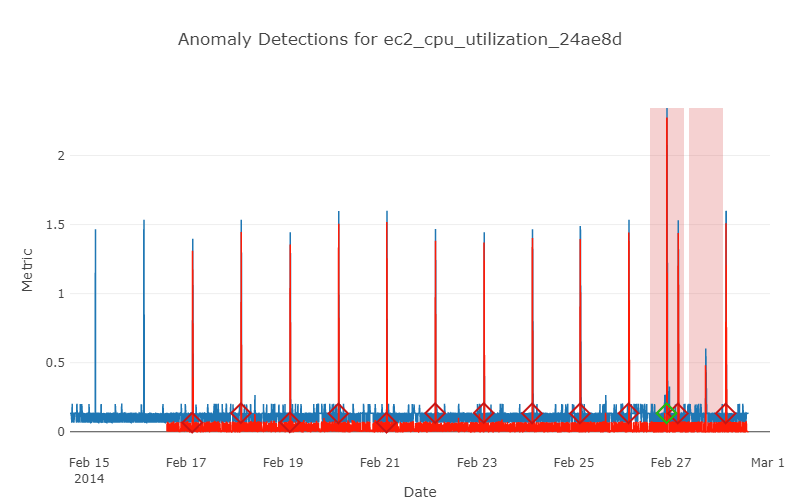
\includegraphics[width=.7\textwidth]{evaluation/deepant/resembles_original2.png}
        \subcaption{A result from DeepAnT from a time series with regular spikes.
        The predicted values (red) closely resemble the original values (blue --- 
        mostly hidden underneath the red predictions).}\label{fig:deepant-resemble}
    \end{subfigure}
\end{figure}
\begin{figure}[htp!]
    \ContinuedFloat{}
    \begin{subfigure}[b]{\linewidth}
        \centering
        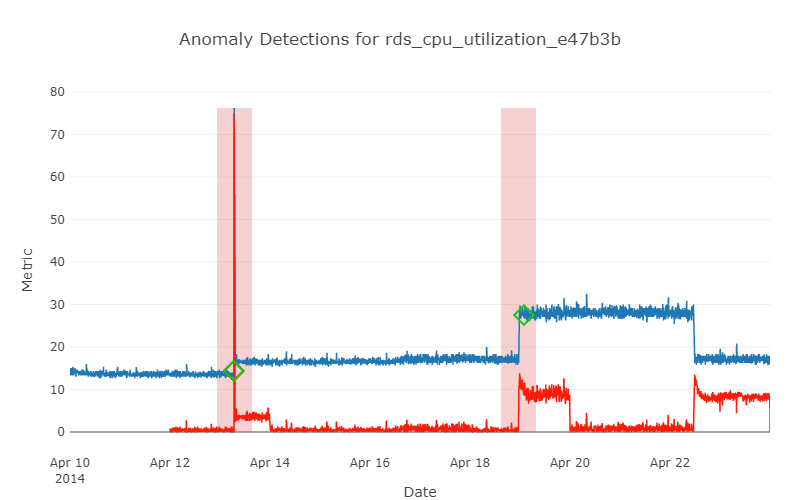
\includegraphics[width=.7\textwidth]{evaluation/deepant/changepoint_response.png}
        \subcaption{DeepAnTs response to multiple changepoints. First, predictions
        occur mean shifted. However, DeepAnT quickly adapts to the new behavior.}\label{fig:deepant-changepoint}
    \end{subfigure}
    \caption{Examples from DeepAnT.}\label{fig:deepant-output}
\end{figure}

\begin{figure}[htp!]
    \begin{subfigure}[b]{\linewidth}
        \centering
        \includegraphics[width=.7\textwidth]{evaluation/nbeats/noisy2.png}
        \subcaption{An example of N-BEATS' lack of sensitivity to long-term cyclicity}\label{fig:nbeats-cyclicity}
    \end{subfigure}
    \\
    \begin{subfigure}[b]{\linewidth}
        \centering
        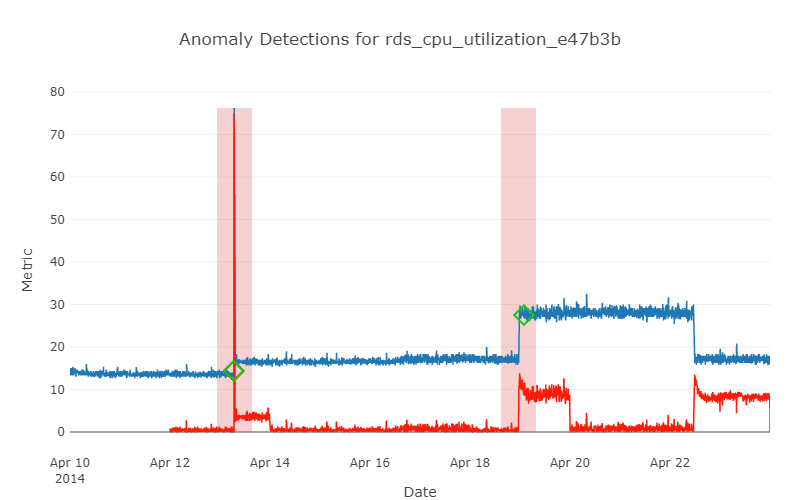
\includegraphics[width=.7\textwidth]{evaluation/deepant/changepoint_response.png}
        \subcaption{Like DeepAnT, output from N-BEATS often resembles the original
        time series.}\label{fig:nbeats-resembles}
    \end{subfigure}
    \\
    \begin{subfigure}[b]{\linewidth}
        \centering
        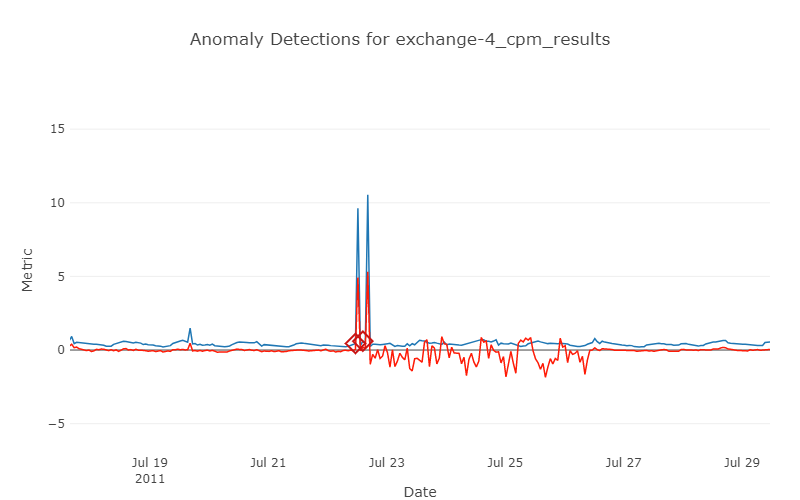
\includegraphics[width=.7\textwidth]{evaluation/nbeats/lasting_impact.png}
        \subcaption{Example of a value spike (Jul 23) that decreases prediction
        accuracy for almost four consecutive day.}\label{fig:nbeats-spike-impact}
    \end{subfigure}
    \caption{Examples from N-BEATS.}\label{fig:nbeats-output}
\end{figure}

\begin{figure}[htp!]
    \begin{subfigure}[b]{\linewidth}
        \centering
        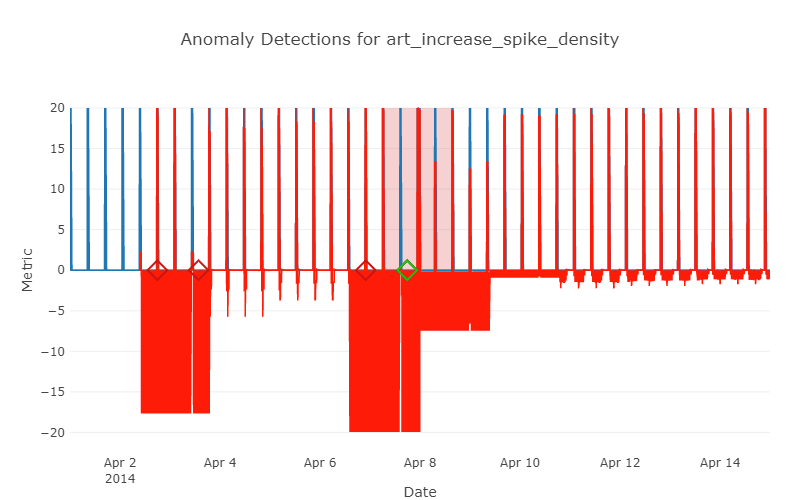
\includegraphics[width=.7\textwidth]{evaluation/hw/broken.png}
        \subcaption{An example of computational instability from Holt-Winters.}\label{fig:hw-broken}
    \end{subfigure}
    \\
    \begin{subfigure}[b]{\linewidth}
        \centering
        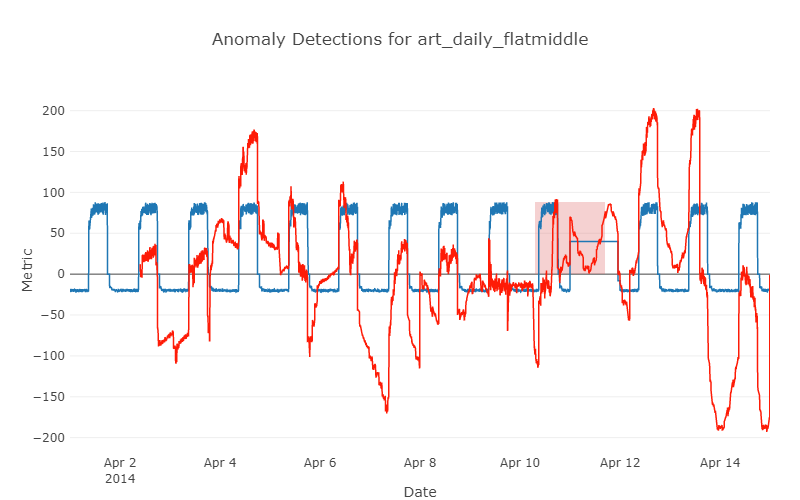
\includegraphics[width=.7\textwidth]{evaluation/hw/broken_trend.png}
        \subcaption{An example of inferred trends from Holt-Winters that are not
        found within the data.}\label{fig:hw-trend-instability}
    \end{subfigure}
    \\
    \begin{subfigure}[b]{\linewidth}
        \centering
        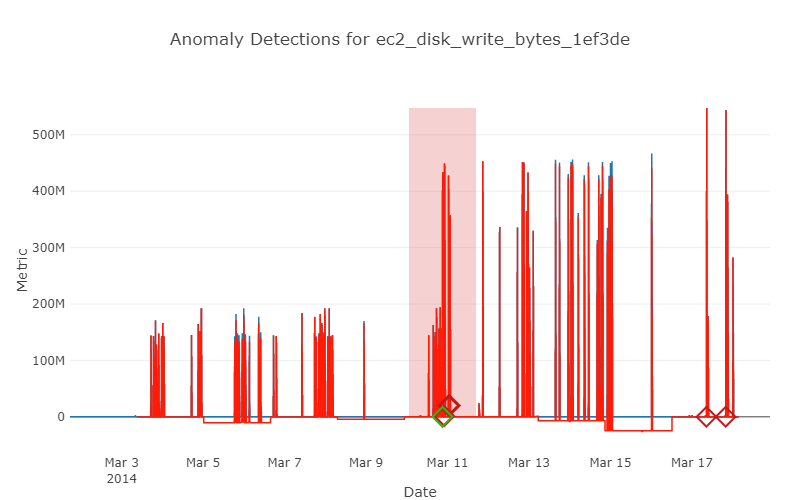
\includegraphics[width=.7\textwidth]{evaluation/hw/unstable3.png}
        \subcaption{A more ordinary example from Holt-Winters.}\label{fig:hw-ordinary}
    \end{subfigure}
    \caption{Examples from Holt-Winters.}\label{fig:hw-output}
\end{figure}

\begin{figure}[htp!]
    \begin{subfigure}[b]{\linewidth}
        \centering
        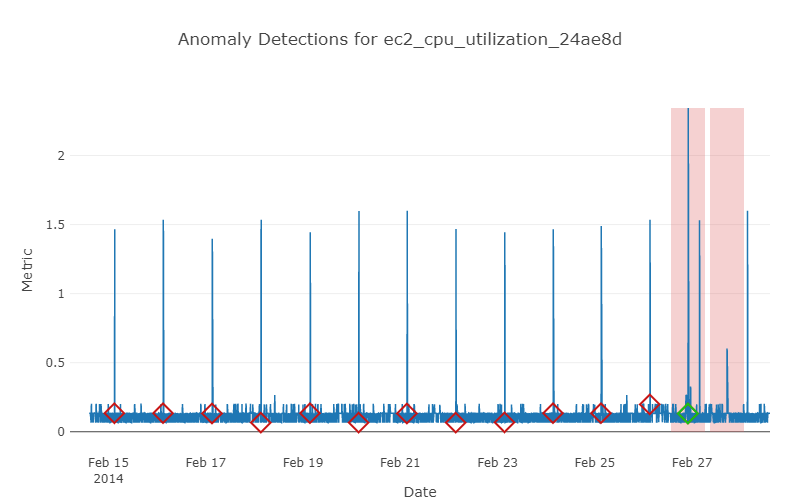
\includegraphics[width=.7\textwidth]{evaluation/arima_khundman/high_fp3.png}
        \subcaption{High false positives rate on time series with many spikes.}\label{fig:arima-fp}
    \end{subfigure}%
    \\
    \begin{subfigure}[b]{\linewidth}
        \centering
        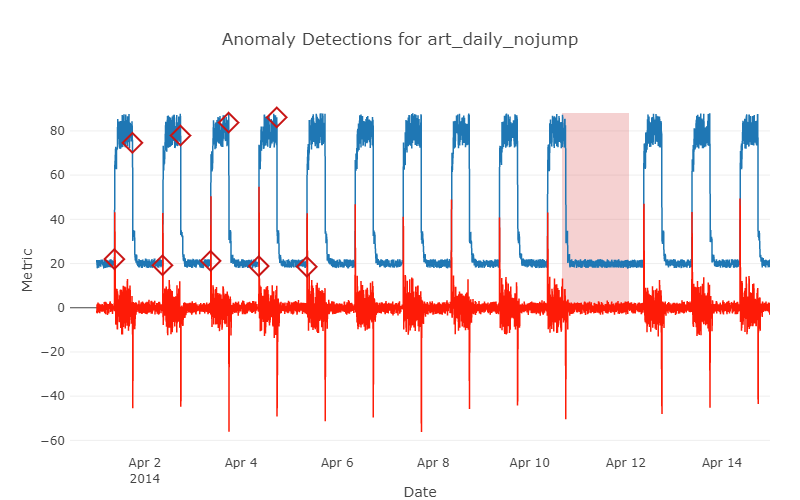
\includegraphics[width=.7\textwidth]{evaluation/arima_khundman/cyclicity2.png}
        \subcaption{ARIMA is unable to adopt long-term cyclicity.}\label{fig:arima-cyclicity}
    \end{subfigure}
    \\
    \begin{subfigure}[b]{\linewidth}
        \centering
        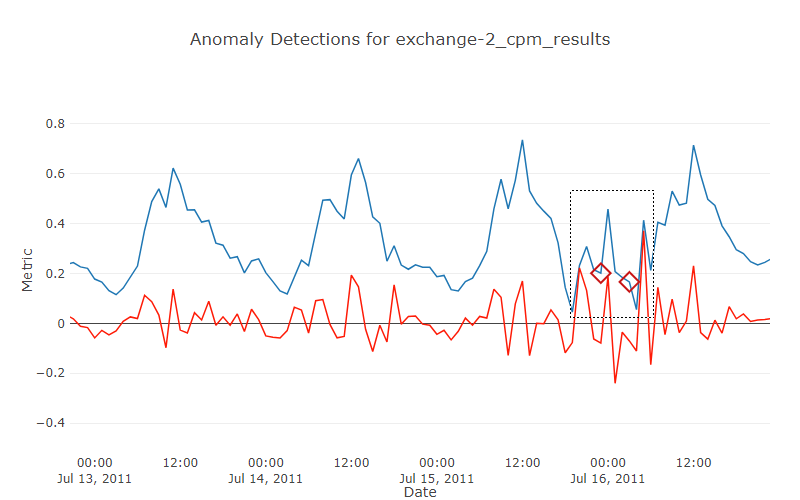
\includegraphics[width=.7\textwidth]{evaluation/arima_khundman/subtle_irregularities_box.png}
        \subcaption{Time series values are colored blue, while algorithm output
        is red. The pattern (dotted box) from the time series deviates from previous
        time steps.}\label{fig:arima-subtle}
    \end{subfigure}
\end{figure}
\begin{figure}[htp!]
    \ContinuedFloat{}
    \begin{subfigure}[b]{\linewidth}
        \centering
        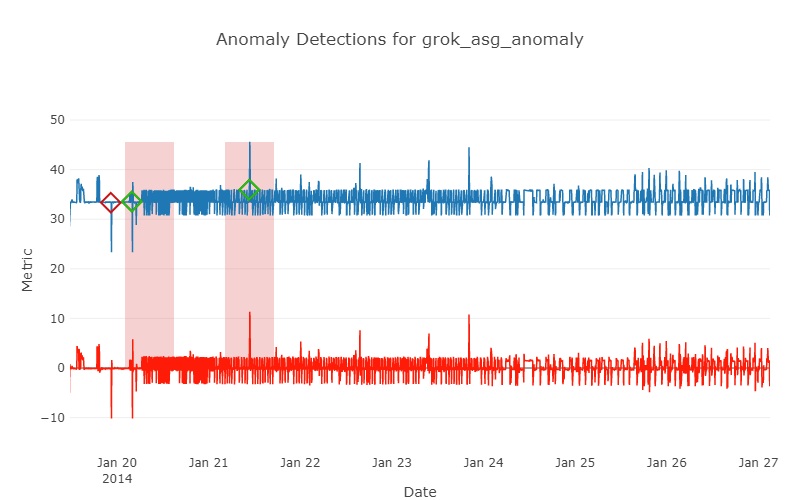
\includegraphics[width=.7\textwidth]{evaluation/arima_khundman/resembles_output3.png}
        \subcaption{On more chaotic time series, output from ARIMA closely
        resembles the original time series.}\label{fig:arima-resembles}
    \end{subfigure}
    \caption{Examples from Auto-ARIMA.}\label{fig:arima-output}
\end{figure}

\begin{figure}[htp!]
    \begin{subfigure}[b]{\linewidth}
        \centering
        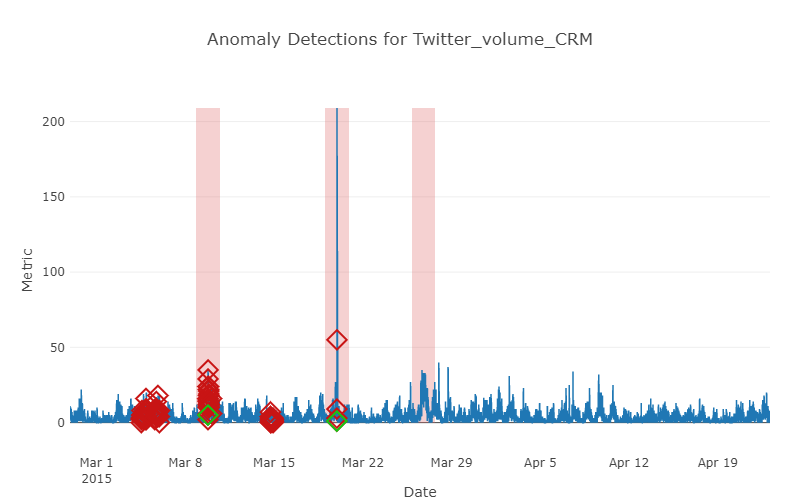
\includegraphics[width=.7\textwidth]{evaluation/prophet/high_fp5.png}
        \subcaption{57 false positives on a single time series.}\label{fig:prophet-fp}
    \end{subfigure}%
    \\
    \begin{subfigure}[b]{\linewidth}
        \centering
        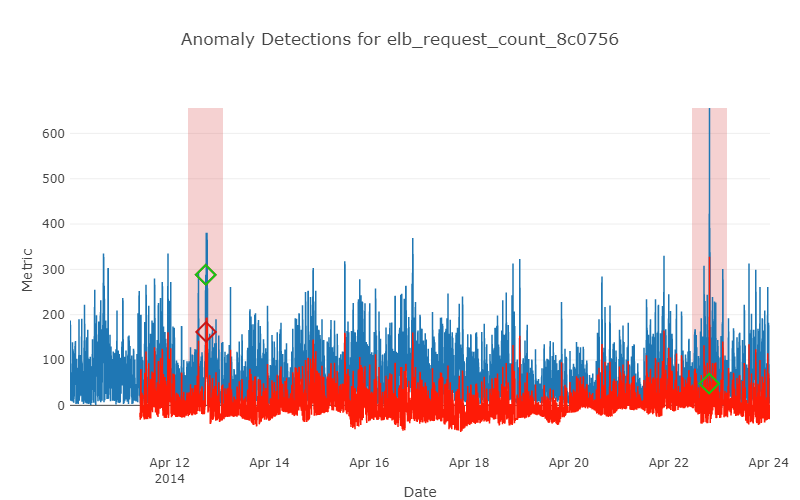
\includegraphics[width=.7\textwidth]{evaluation/prophet/noisy_low_fp.png}
        \subcaption{Prophet often assumed seasonality within the data, producing
        a curvy output.}\label{fig:prophet-curvy}
    \end{subfigure}
    \\
    \begin{subfigure}[b]{\linewidth}
        \centering
        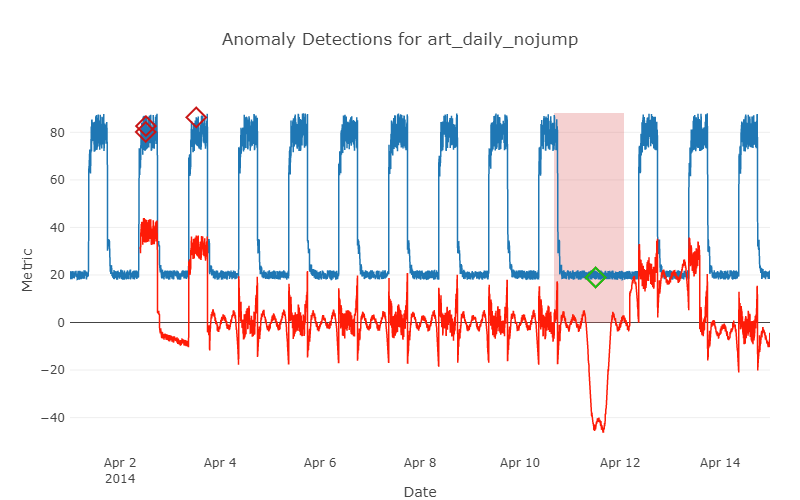
\includegraphics[width=.7\textwidth]{evaluation/prophet/cyclicity3.png}
        \subcaption{Successful adaptation to the cyclicity of a simple time series.}\label{fig:prophet-cyclicity}
    \end{subfigure}
\caption{Examples from Prophet.}\label{fig:prophet-output}
\end{figure}
\clearpage

\section{Illustrations from Boundary Algorithms}

\begin{figure}[htp!]
    \begin{subfigure}[b]{\linewidth}
        \centering
        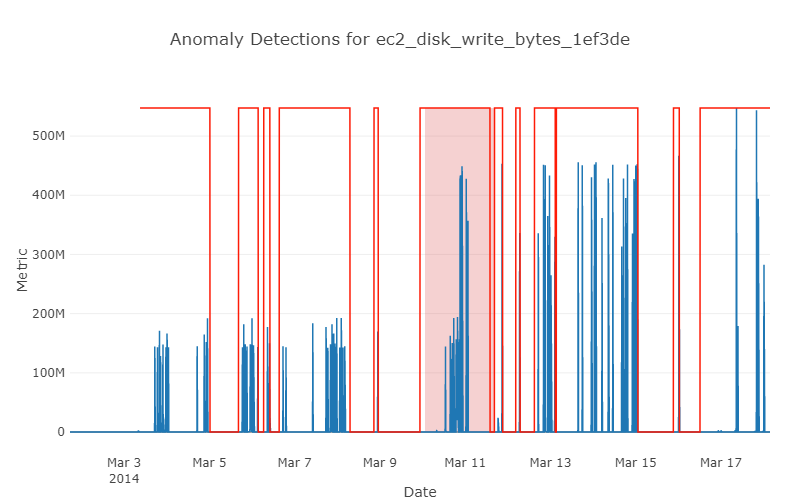
\includegraphics[width=.7\textwidth]{evaluation/ocsvm/noisy1.png}
        \subcaption{Output from \gls{ocsvm} seems to lay \textit{boxes} around
        observations with value \(> 0\). Useless output for the task of anomaly
        detection.}
    \end{subfigure}%
    \\
    \begin{subfigure}[b]{\linewidth}
        \centering
        \includegraphics[width=.7\textwidth]{evaluation/ocsvm/noisy2.png}
        \subcaption{In this example, \gls{ocsvm} claims every that every 
        observation is anomalous.}
    \end{subfigure}
    \caption{Unusable outputs from \gls{ocsvm}. Blue lines represent observations
    from the time series. Red lines represent the output from \gls{ocsvm}.
    Illustration by the author.}\label{fig:ocsvm-output}
\end{figure}

\begin{figure}[htp!]
    \begin{subfigure}[b]{\linewidth}
        \centering
        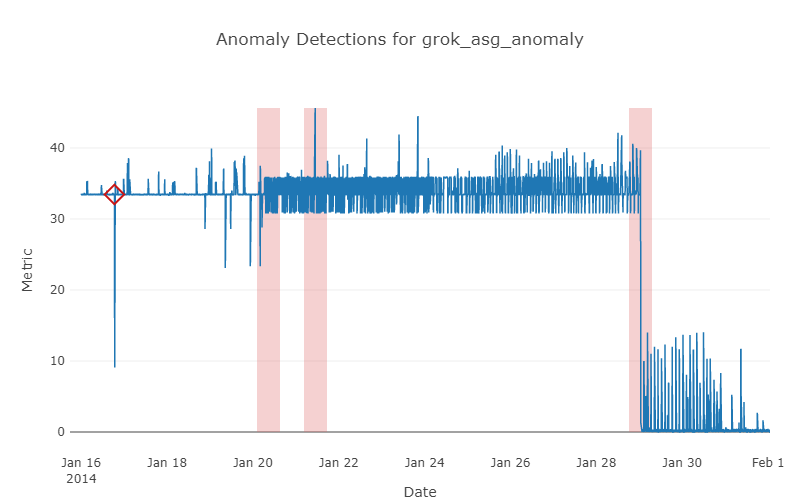
\includegraphics[width=.7\textwidth]{evaluation/lof/no_detection.png}
        \subcaption{Output from \gls{lof}, where no detections are produced on
        a seemingly simple example. Anomalous time windows are marked red.}
    \end{subfigure}%
    \\
    \begin{subfigure}[b]{\linewidth}
        \centering
        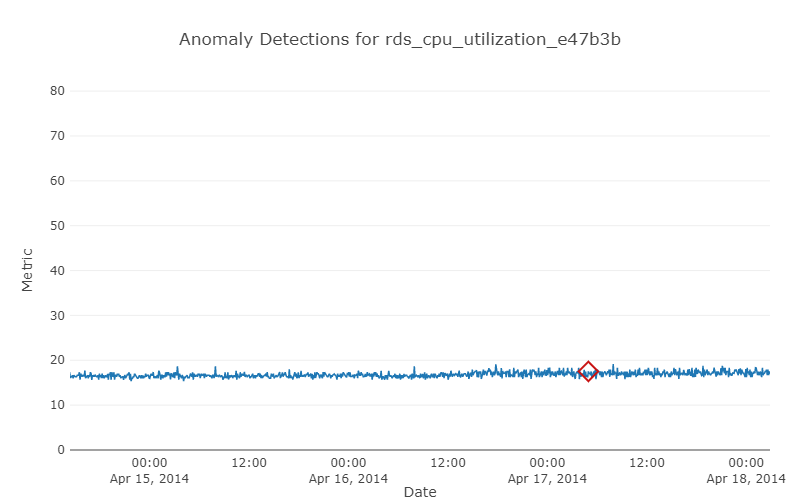
\includegraphics[width=.7\textwidth]{evaluation/lof/unreasonable_detection2.png}
        \subcaption{Example of an unreasonable detection by \gls{lof}.}
    \end{subfigure}
\end{figure}

\begin{figure}[htp!]
    \ContinuedFloat{}
    \begin{subfigure}[b]{\linewidth}
        \centering
        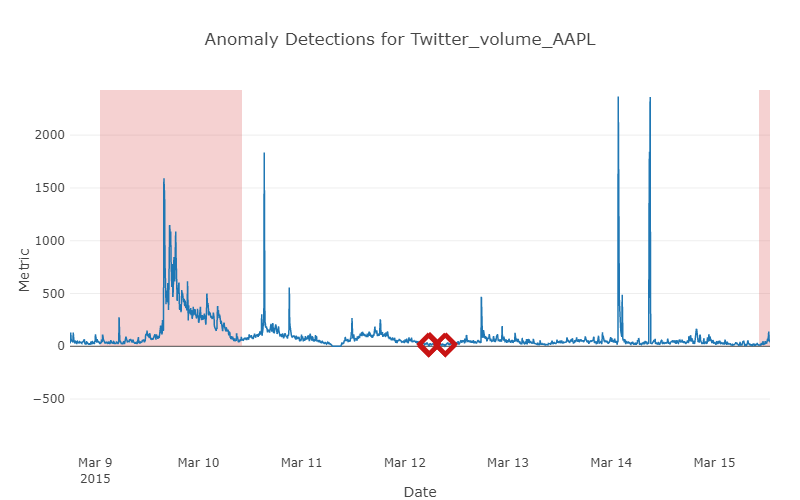
\includegraphics[width=.7\textwidth]{evaluation/lof/unreasonable_detection3.png}
        \subcaption{Another example of an unreasonable detection by \gls{lof}.}
    \end{subfigure}
    \caption{(Seemingly) unreasonable detections from \gls{lof}. Detections are
    depicted as colored diamond symbols. Illustration by the author.}\label{fig:lof-output}
\end{figure}

\begin{figure}[htp!]
    \begin{subfigure}[b]{\linewidth}
        \centering
        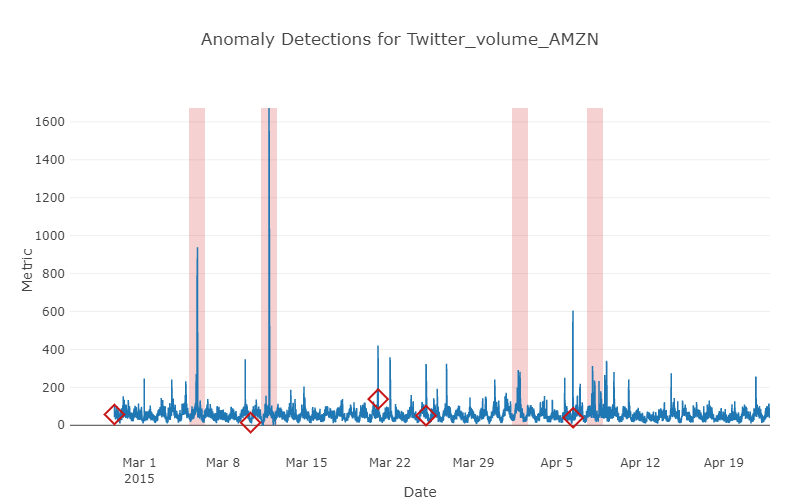
\includegraphics[width=.7\textwidth]{evaluation/dagmm/no_tp.png}
        \subcaption{False positives from \gls{dagmm}}
    \end{subfigure}%
    \\
    \begin{subfigure}[b]{\linewidth}
        \centering
        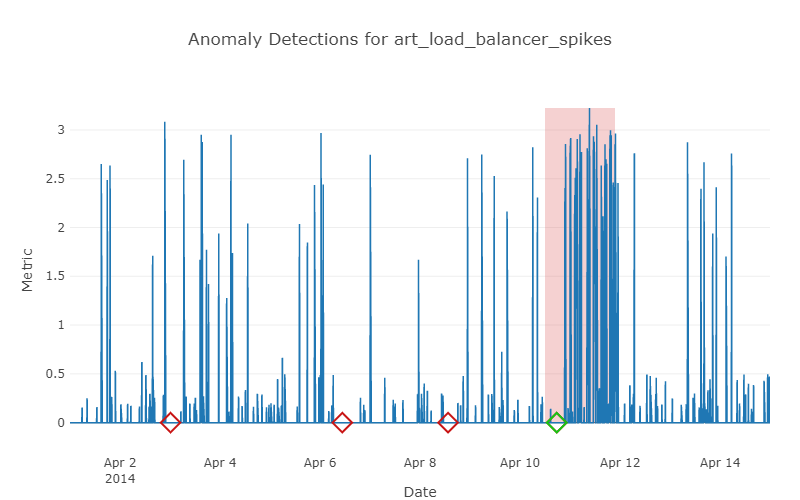
\includegraphics[width=.7\textwidth]{evaluation/dagmm/lucky_detections.png}
        \subcaption{A representative true positive from \gls{dagmm}. The
        reason for the anomaly is the high value spike (inside the red area).
        \gls{dagmm} (unreasonably) attributes the anomaly to a normal value
        approximately two days previous.}
    \end{subfigure}
    \caption{Examples from \gls{dagmm}.}\label{fig:dagmm-output}
\end{figure}

\begin{figure}[htp!]
    \begin{subfigure}[b]{\linewidth}
        \centering
        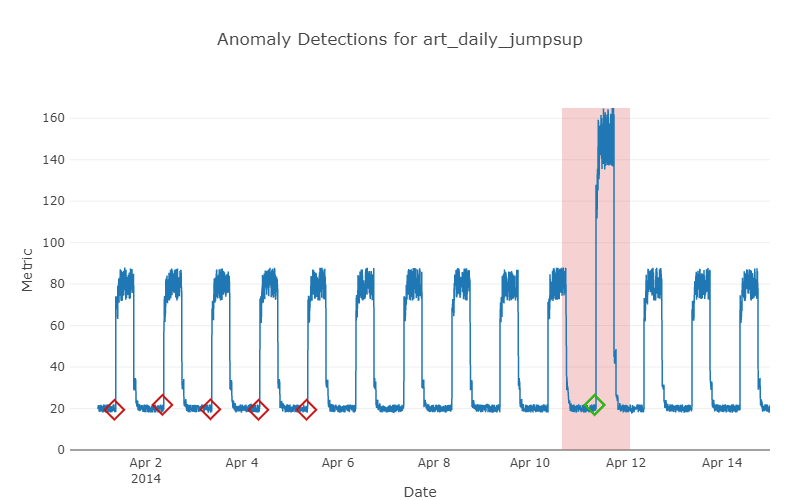
\includegraphics[width=.7\textwidth]{evaluation/rrcf/season1.png}
        \subcaption{Example detection of a cyclicity violation. True positives
        are displayed as green- and false positives as red diamonds.}
    \end{subfigure}%
    \\
    \begin{subfigure}[b]{\linewidth}
        \centering
        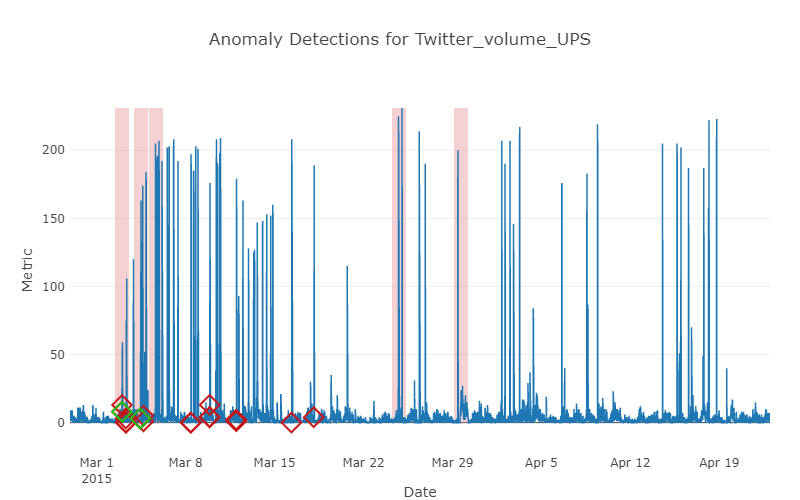
\includegraphics[width=.7\textwidth]{evaluation/rrcf/confused3.png}
        \subcaption{A representative result from \gls{rrcf}, where a complex
        time series confuses the algorithm.}
    \end{subfigure}
    \caption{Examples from \gls{rrcf}.}\label{fig:rrcf-output}
\end{figure}

\begin{figure}[htp!]
    \begin{subfigure}[b]{\linewidth}
        \centering
        \includegraphics[width=.7\textwidth]{evaluation/khundman/highfp.png}
        \subcaption{High false positives rate on time series with many spikes.}\label{fig:khundman-fp}
    \end{subfigure}%
    \\
    \begin{subfigure}[b]{\linewidth}
        \centering
        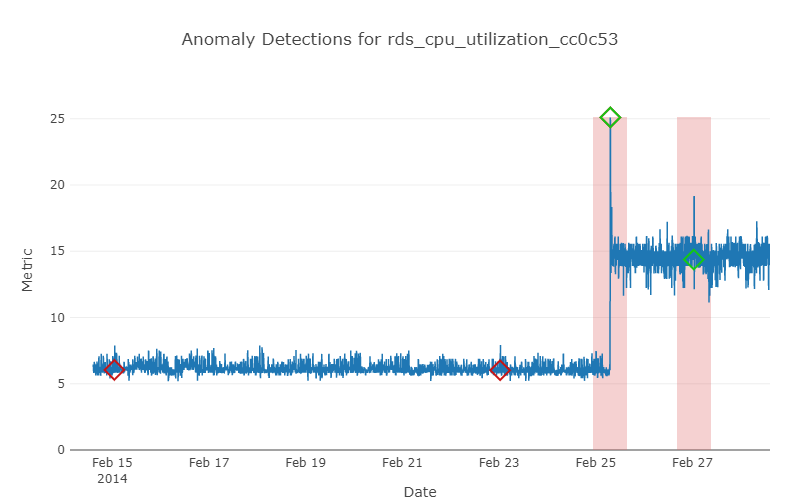
\includegraphics[width=.7\textwidth]{evaluation/khundman/success.png}
        \subcaption{Successful detection of two spikes.}\label{fig:khundman-success}
    \end{subfigure}
    \caption{Examples from \gls{ndt}.}\label{fig:khundman-output}
\end{figure}

\begin{figure}[htp!]
    \begin{subfigure}[b]{\linewidth}
        \centering
        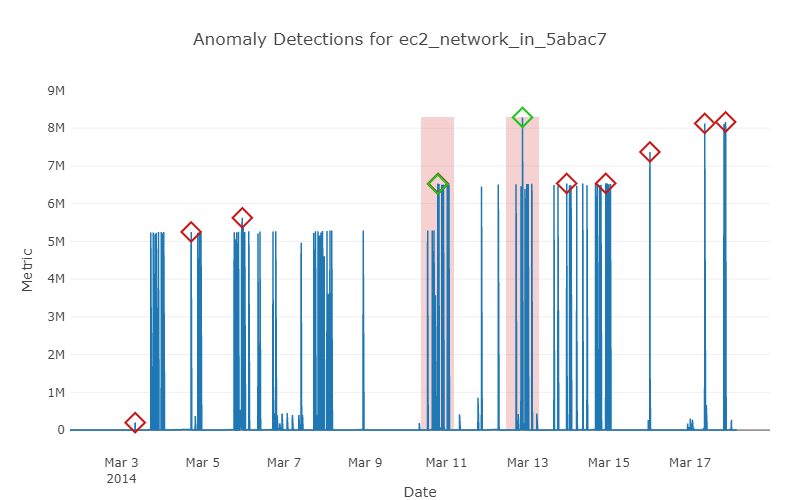
\includegraphics[width=.7\textwidth]{evaluation/lstm_ad/false-positives.png}
        \subcaption{High false positives rate on time series with many spikes.}\label{fig:lstmad-fp}
    \end{subfigure}%
    \\
    \begin{subfigure}[b]{\linewidth}
        \centering
        \includegraphics[width=.7\textwidth]{evaluation/lstm_ad/cyclicity.png}
        \subcaption{Cyclicity violations remain undetected by LSTM-AD.}\label{fig:lstmad-cyclicity}
    \end{subfigure}
    \caption{Examples from LSTM-AD.}\label{fig:lstmad-output}
\end{figure}

\begin{figure}[htp!]
    \begin{subfigure}[b]{\linewidth}
        \centering
        \includegraphics[width=.7\textwidth]{evaluation/cblof/highfp.png}
        \subcaption{High false positives rate on (some) time series with irregular spikes.}\label{fig:cblof-fp}
    \end{subfigure}%
    \\
    \begin{subfigure}[b]{\linewidth}
        \centering
        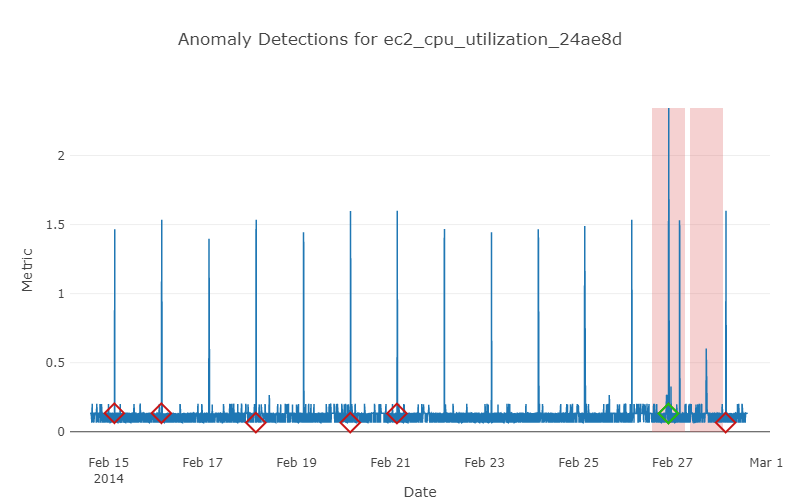
\includegraphics[width=.7\textwidth]{evaluation/cblof/infreq_spikes.png}
        \subcaption{Adaptation to more regularly spiking time series.}\label{fig:cblof-cyclicity}
    \end{subfigure}
\end{figure}

\begin{figure}[htp!]
    \ContinuedFloat{}
    \begin{subfigure}[b]{\linewidth}
        \centering
        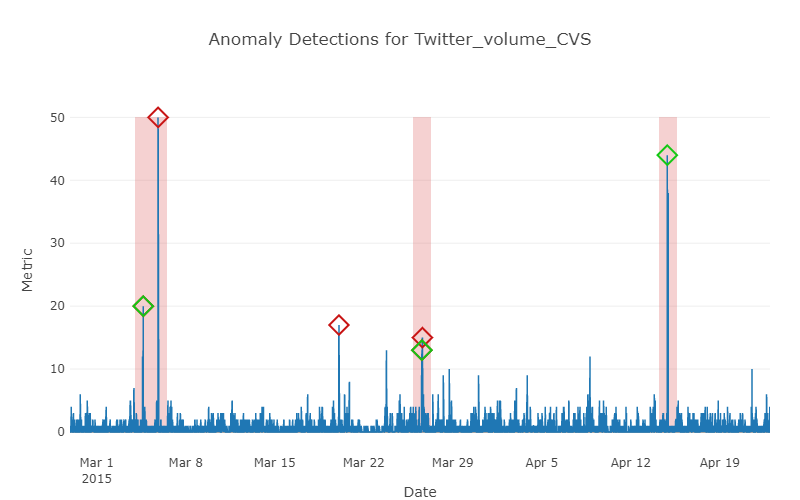
\includegraphics[width=.7\textwidth]{evaluation/cblof/good_result.png}
        \subcaption{Example of a good result from \gls{cblof}.}\label{fig:cblof-good}
    \end{subfigure}
\caption{Examples from \gls{cblof}.}\label{fig:cblof-output}
\end{figure}


\begin{figure}[htp!]
    \begin{subfigure}[b]{\linewidth}
        \centering
        \includegraphics[width=.7\textwidth]{evaluation/lstm_ed/highfp.png}
        \subcaption{High false positives rate on (some) time series with irregular spikes.}\label{fig:lstmed-fp}
    \end{subfigure}%
    \\
    \begin{subfigure}[b]{\linewidth}
        \centering
        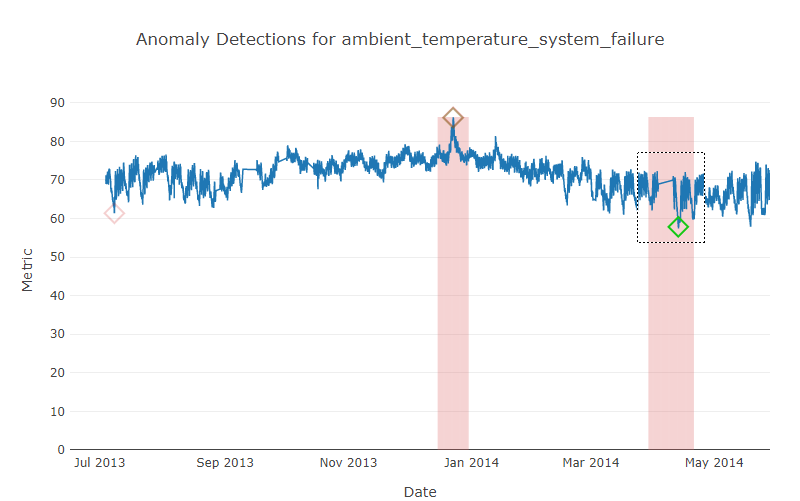
\includegraphics[width=.7\textwidth]{evaluation/lstm_ed/harder_box.png}
        \subcaption{A harder anomaly (dotted box) detected by LSTM-ED.}\label{fig:lstmed-harder}
    \end{subfigure}
    \\
    \begin{subfigure}[b]{\linewidth}
        \begin{subfigure}[b]{.45\linewidth}
            \centering
            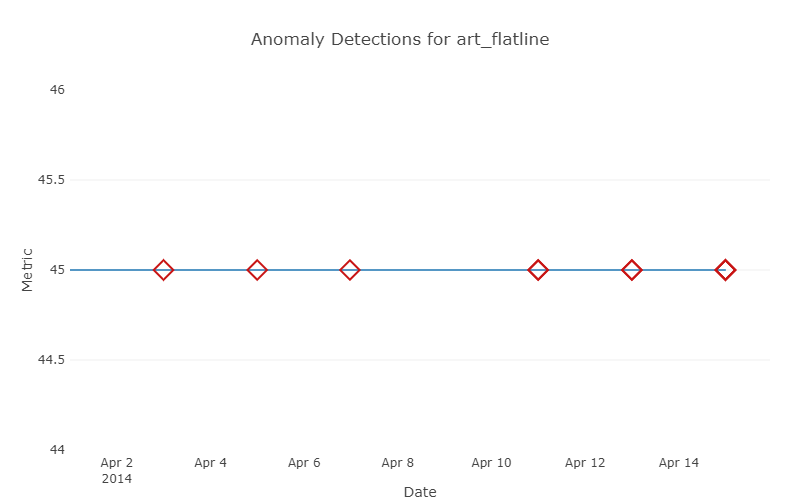
\includegraphics[width=\textwidth]{evaluation/lstm_ed/artificial_lstm.png}
        \end{subfigure}
        \hfill
        \begin{subfigure}[b]{.45\linewidth}
            \centering
            \includegraphics[width=\textwidth]{evaluation/lstm_ed/artificial_cblof.png}
        \end{subfigure}
        \subcaption{Left) Results from LSTM-ED on one of the artificial time series (straight line).
        Right) Results from \gls{cblof} on the same artificial time series.}\label{fig:lstmed-artificial}
    \end{subfigure}
\caption{Examples from LSTM-ED.}\label{fig:lstmed-output}
\end{figure}

\begin{figure}[htp!]
    \begin{subfigure}[b]{\linewidth}
        \centering
        \includegraphics[width=.7\textwidth]{evaluation/knn/cyclicity.png}
        \subcaption{A simple cyclicity violation that was detected by \gls{knn},
        presumably due to its unusual value range.}\label{fig:knn-cyclicity}
    \end{subfigure}%
    \\
    \begin{subfigure}[b]{\linewidth}
        \centering
        \includegraphics[width=.7\textwidth]{evaluation/knn/good.png}
        \subcaption{A difficult anomaly detected by \gls{knn} (rightmost anomaly).}\label{fig:knn-harder}
    \end{subfigure}
\caption{Examples from \gls{knn}.}\label{fig:knn-output}
\end{figure}




\todo{Check if clearpage is still necessary in complete appendix}
\todo{Remove DOI-Links}
\todo{Order figures to their chronology within the text}